\documentclass[11pt]{article}

\usepackage[T2A]{fontenc}
\usepackage[utf8]{inputenc}
\usepackage[russian]{babel}

\usepackage{indentfirst}
\usepackage{geometry}
\usepackage{graphicx}
\usepackage{caption}
\usepackage{subcaption}

\usepackage{amsmath, amssymb, amsfonts, amsthm}
\usepackage{mathrsfs}

\geometry{a4paper}
\sloppy

\theoremstyle{plain}
\newtheorem*{theorem}{Теорема}
\theoremstyle{definition}
\newtheorem*{definition}{Определение}


\renewcommand{\le}{\leqslant}
\renewcommand{\ge}{\geqslant}
\renewcommand{\phi}{\varphi}
\renewcommand{\epsilon}{\varepsilon}

\newcommand*\segm[2]{\left[#1,#2\right]}
\newcommand*\inter[2]{(#1,#2)}
\newcommand*\abs[1]{\left|#1\right|}

\newcommand*\Ind[1]{\mathbb{I}\left(#1\right)}
\newcommand*\Prb[1]{\mathbb{P}\left(#1\right)}

\DeclareMathOperator{\Exp}{\mathbb{E}}
\DeclareMathOperator{\Disp}{\mathbb{D}}
\DeclareMathOperator{\cov}{cov}

\begin{document}

\begin{titlepage}
    \begin{centering}
        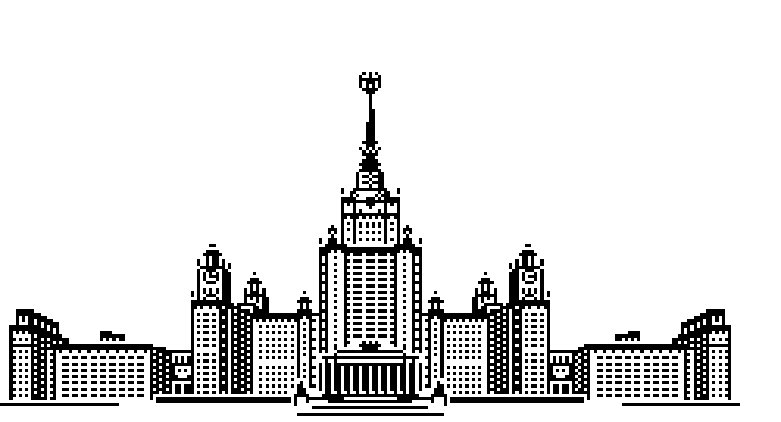
\includegraphics[width=0.5\textwidth]{resources/msu.png}\\
        {\scshape Московский государственный университет имени М.~В.~Ломоносова}\\
        Факультет вычислительной математики и кибернетики\\
        Кафедра системного анализа\\
        \vfill
        {\LARGE Отчет по компьютерному практикуму к курсу}\\
        \vspace{1cm}
        {\Huge\bfseries "<Стохастический анализ и моделирование">\\}
    \end{centering}
    \vspace{1cm}
    \begin{flushright}
        \begin{large}
            {\itshape Студент 415 группы\\}
            А.~А.~Владимиров\\
            \vspace{5mm}
            {\itshape Руководитель практикума\\}
            к.ф.-м.н., доцент С.~Н.~Смирнов\\
        \end{large}
    \end{flushright}
    \vfill
    \begin{centering}
        Москва, 2022\\ 
    \end{centering}
\end{titlepage}

\newpage
\setcounter{page}{2}
\tableofcontents
\newpage

\section{Задание 1}
    Считается доступным лишь генератор равномерно распределенной на 
    отрезке \(\segm{0}{1}\) случайной величины
    $\eta \sim \mathrm{Uni}\inter{0}{1}$. Требуется:

    \begin{enumerate}
        \item Реализовать генератор схемы Бернулли с заданной вероятностью
        успеха $p$. На основе генератора схемы Бернулли построить датчик для
        биномиального распределения.
        \item Реализовать генератор геометрического распределения. Проверить 
        для данного распределения свойство отсутствия памяти.
        \item Рассмотреть игру в орлянку~--- бесконечную последовательность 
        независимых испытаний с бросанием правильной монеты. Выигрыш $S_n$ 
        определяется как сумма по всем $n$ испытаниями $1$ и $-1$ в зависимости 
        от выпавшей стороны. Проиллюстрировать (в виде ломанной) поведение 
        нормированной суммы $Y(i) = S_i/\sqrt{n}$, как функцию от номера 
        испытания $i = 1,\dots, n$ для одной отдельно взятой траектории. Дать 
        теоритическую оценку для $Y(n)$  при $n \rightarrow \infty$.
    \end{enumerate}

    \subsection{Реализация схемы Бернулли и биномиального распределения}
        Под схемой Бернулли понимается серия однородных независимых испытаний, 
        каждое из которых с вероятностью $p$ оканчивается успехом или, с 
        вероятностью $q = 1-p$, неудачей.

        Чтобы практически реализовать схему Бернулли нужно получить н.о.р.с.в.\\ 
        $\xi_i \sim \mathrm{Bern}(p), i = 1,\dots,n$. Для этого достаточно 
        выразить $\xi_i$ через $\eta$ следующим образом: $\xi_i = 
        \Ind{\eta < p} + \Ind{\eta \ge p}$, т.е.

        \[\xi_i = \left\{\begin{aligned}
                            1,&\quad \eta < p,\\
                            0,&\quad \eta \ge p.
        \end{aligned}\right.\]
    
        В свою очередь $\beta \sim \mathrm{Bin}(n,p)$ можно представить как 
        $\beta = \sum\limits_{i=1}^{n} \xi_i$.

        Программа, по описанной выше схеме моделирующая $\mathrm{Bin}(16,0.5)$, 
        дает следующий результат (рис. \ref{task1_bin}).
        
    \subsection{Геометрическое распределение} \label{par12}
        Под геометрическим распределением подразумевают распределение случайной 
        величины $\gamma$ равной числу неудач до первого успеха в серии 
        испытаний Бернулли. $\Prb{\gamma = n} = q^n p$.

        Случайная величина $\gamma \sim \mathrm{Geom}(p)$ представима как 
        \[\gamma = \max\{n \in \mathbb{N} \cup \{0\} : 
        \xi_i = 0,\:i = 1,\ldots,n\}.\]

        Геометрическое распределение обладает свойством отсутствия памяти, т.е.

        \[\mathbb{P}(\gamma > m + n \mid \gamma \ge m) = \mathbb{P}(\gamma > n), 
        \quad\forall{m,n} \in \mathbb{N} \cup \{0\}.\]

        Это свойство можно переформулировать. Пусть 
        $\gamma~\sim~\mathrm{Geom}(p)$~--- случайная величина, определенная на 
        вероятностном пространстве $\left(\Omega,\mathcal{A},\mathbb{P}\right)$.
        Свойство отсутствия памяти сл. в. $\gamma$ означает, что
        \smallskip

        \[\bigl. \gamma_m \sim \gamma ,\quad 
        \forall{m} \in \mathbb{N} \cup \{0\},\]
        где $\gamma_m := (\gamma \bigr|_{\Omega_m} - m), 
        \quad \Omega_m = \gamma^{-1}(\gamma \geqslant m) \in \mathcal{A}.$ 

        То есть для каждого $m$ распределение случайной величины $\gamma$ 
        отличается ровно на константу $m$ от распределения сл.в. $\gamma$, 
        индуцированной на вероятностное подпространство $\Omega_m$.

        Проверка свойства отсутствия памяти проведена численным моделированием 
        распределений сл.в. $\gamma$ и $\gamma_m$ (рис. \ref{task1_memo}).
        
        \begin{figure}[tbp]
            \centering
            \begin{subfigure}[b]{0.4\textwidth}
                \centering
                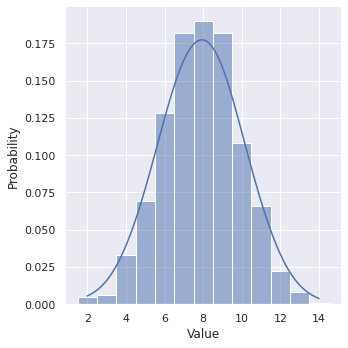
\includegraphics[width=\textwidth]{resources/task1_bin.png}
                \caption{Биномиальное распределение}
                \label{task1_bin}
            \end{subfigure}
            \hfill
            \begin{subfigure}[b]{0.5\textwidth}
                \centering
                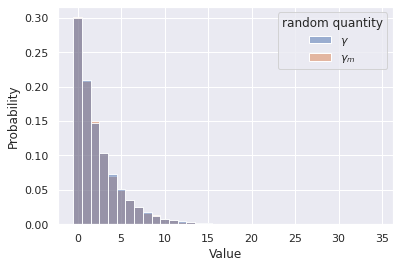
\includegraphics[width=\textwidth]{resources/task1_memo.png}
                \caption{Отсутствие памяти ($m = 5$)}
                \label{task1_memo}
            \end{subfigure}
            \caption{}
        \end{figure}


    \subsection{Игра в орлянку}
        Даны $n$ н.о.р.с.в.

        \[\theta_j: \mathbb{P}(\theta_j = 1 ) = \mathbb{P}(\theta_j = -1) 
                                          = \frac{1}{2}, \quad j = 1,\ldots,n.\]

        Рассматривается нормированная сумма

        \[Y(i) = \frac{S_i}{\sqrt{n}},\quad \text{где } 
                                       S_i = \sum\limits_{j = 1}^{n} \theta_j,\]

        пример поведения которой проиллюстрирован на рис. \ref{task1_toss}.

        \bigskip

        \begin{figure}[tbp]
            \centering
            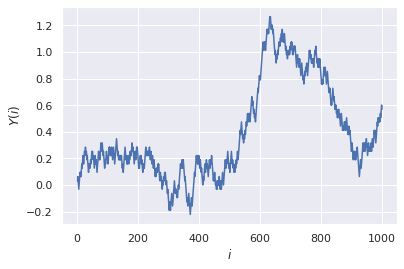
\includegraphics[width=0.5\textwidth]{resources/task1_toss.png}
            \caption{Игра в орлянку ($n = 1000$)}
            \label{task1_toss}
        \end{figure}

        Для оценки $Y(n)$ при $n \rightarrow \infty$, нам потребуется
        \begin{theorem}[Центральная предельная теорема]
            Пусть $\xi_1, \xi_2, \ldots$~--- последовательность независимых 
            одинаково распределенных (невырожденных) случайных величин с 
            $\Exp{\xi_1^2} \le \infty$ и $S_n = \xi_1 + \ldots + \xi_n$. Тогда
            \[\frac{S_n - \Exp{S_n}}{\sqrt{\Disp{S_n}}} 
            \stackrel{d}{\longrightarrow} \mathrm{Norm}(0,1).\]   
        \end{theorem}

        Действительно

        \[\frac{S_n - \Exp{S_n}}{\sqrt{\Disp{S_n}}} = 
        \frac{S_n - 0}{\sqrt{n\Disp{\theta_1)}}} = \frac{S_n}{\sqrt{n}} = Y(n) 
        \stackrel{d}{\longrightarrow} \mathrm{Norm}(0,1).\]
        
\section{Задание 2}
    \begin{enumerate}
        \item Построить датчик сингулярного распределения, имеющий в качестве 
        функции распределения канторову лесницу. С помощью критерия Колмогорова 
        убедиться в корректности работы датчика.
        \item Для канторовых случайных величин проверить свойство симметричности 
        относительно $\frac{1}{2}$ ($X$ и $1 - X$ распределены одинаково) и 
        самоподобия относительно деления на 3 (условное распределение $Y$ при 
        условии $Y \in \segm{0}{\frac{1}{3}}$ совпадает с распределением 
        $Y/3$) с помощью критерия Смирнова.
        \item Вычислить значение математического ожидания и дисперсии для 
        данного распределения. Сравнить теоретические значения с эмпирическими 
        для разного объема выборок. Проиллюстрировать сходимость.
    \end{enumerate}

    \subsection{Датчик для канторова распределения}
        Случайная величина имеет канторово распеделение, если ее функция 
        распределения~--- канторова лестница.

        Носителем канторова распределения является канторово множество, 
        представимое как счетное пересечение множеств

        \begin{align*}
            C_0 = {} & [0,1] \\
            C_1 = {} & [0,1/3] \cup [2/3,1] \\
            C_2 = {} & [0,1/9] \cup [2/9,1/3] \cup [2/3,7/9] \cup [8/9,1] \\
            \cdots, & \\
            C_n = & \bigcup_{i = 1,\ldots, 2^n}{\segm{a_i}{b_i}}
        \end{align*}

        Причем $\Prb{\segm{a_i}{b_i}} = \dfrac{1}{2^n},\:\forall i$, что дает 
        естественный способ разложения сл.в. $\delta~\sim~\mathrm{Cant}$ в ряд 
        по  $\xi~\sim~\mathrm{Bern(0.5)}$

        \begin{equation}\label{cauchy_series}
            \delta = \sum\limits_{i = 1}^{\infty} \dfrac{2}{3^i}\xi_i.
        \end{equation}

        Таким образом, для моделирования канторовской случайной величины 
        достаточно провести достаточно большое число испытаний бернулли и 
        посчитать сумму приближающую ряд \eqref{cauchy_series}.

        \begin{figure}[tbp]
            \centering
            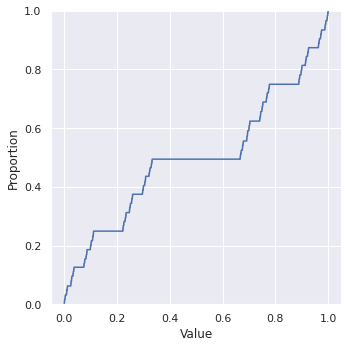
\includegraphics[width=0.5\textwidth]{resources/task2_cantor.png}
            \caption{Э.ф.р. канторовой сл.в.}
            \label{task1_cantor}
        \end{figure}
        
        \bigskip
        
        Для проверки корректности полученного датчика напомним следующee.

        Статистикой критерия Колмогорова является величина 
        \[\sqrt{n}D_n = \sup\limits_{-\infty < x < \infty} 
                                                \abs{\widehat F_n(x) - F(x)},\]
        где $\widehat F_n(x) = \dfrac{1}{n}\sum\limits_{i=1}^{n} 
        \Ind{X_i \le x}$~--- эмпирическая функция распределения.

        \begin{theorem}[Колмогоров] Если функция распределения элементов выборки 
            $F(x)$ непрерывна, то для $x > 0$
            \[\lim_{n\rightarrow\infty}\Prb{\sqrt{n}D_n \le x} = K(x) = 
            1 + 2\sum\limits_{k=1}^{\infty}(-1)^k e^{-2k^2 x^2}.\]
        \end{theorem}

        Проверяемая гипотеза c заданным \emph{уровнем значимости $\alpha$} 
        отвергается, если на полученной выборке $(X_1,\ldots,X_n)$ значение 
        статистики неправдоподобно велико, т.е.
        \begin{equation}\label{rej_cond}
            \sqrt{n}D_n(X_1,\ldots,X_n) \ge x_{1-\alpha},
        \end{equation}
        где $x_{1-\alpha}$~--- наименьшее значение, удовлетворяющее условию
        \[\Prb{\sqrt{n}D_n \ge x_{1-\alpha}} \le \alpha.\]

        В силу теоремы Колмогорова ``в пределе'' 
        \[\Prb{\sqrt{n}D_n \ge x_{1-\alpha}} = 1 - K(x_{1-\alpha}) = 
                                                    1 - (1-\alpha) = \alpha,\]
        и $\: x_{1-\alpha}$ есть не что иное как $(1-\alpha)$-квантиль функции 
        $K(x)$.                                                    

        Таким образом для значения статистики $\sqrt{n}D_n(X)$ на некоторой 
        определенной выборке $X$ справедливо

        \[\Prb{\sqrt{n}D_n \ge \sqrt{n}D_n(X)} = 1 - K(\sqrt{n}D_n(X)) = 
        1 - (1-\alpha(X)) = \alpha(X)\]

        тем самым $\sqrt{n}D_n$~--- $(1-\alpha(X))$-квантиль, и условие 
        \eqref{rej_cond} выполнено для тех и только тех $x_{1-\alpha}$, что 
        \begin{gather*}
            x_{1-\alpha(X)} \ge x_{1-\alpha} \Leftrightarrow \\
            1-\alpha(X) \ge 1-\alpha \Leftrightarrow \\
            \alpha \ge \alpha(x)
        \end{gather*}

        Выходит что для полученной в результате серии испытаний статистики 
        $\sqrt{n}D_n(X)$ значение $1 - K(\sqrt{n}D_n(X)) = \alpha(X)$ означает, 
        что гипотезу \emph{следует отвергнуть} тогда и только тогда, когда был 
        принят уровень значимости $\alpha$ больший чем величина $\alpha(X)$. И 
        обратно, гипотеза \emph{может быть принята} для любого уровня значимости 
        $\alpha$ меньшего чем $\alpha(X).$
        
        Поскольку функция $F(x)$ непрерывна и не убывает, а $\hat F_n(x)$~--- 
        кусочно-постоянна, то $D_n$ можно вычислить по формуле
        
        \[D_n(x_1,\ldots,x_n) = \max\limits_{1\le i \le n}
        \left\{\dfrac{1}{n} - F(x_{(i)}),\: F(x_{(i)}) - \dfrac{i-1}{n}\right\}.\]

        Посчитанная таким образом на некотрой выборке $(X_1,\ldots,X_n)$ 
        значений датчика $\delta$ статистика $D_n$ составляет приблизительно 
        $0.0087$. Величина $1-K(\sqrt{n}D_n) = \alpha(X)$ равна приблизительно 
        $0.9999$, что даёт нам основания принять гипотезу о корректности 
        построенного датчика $\delta$, с уровнем значимоcти, например, 20\%.

    \subsection{Свойства симметричности и самоподобия}
        Для проверки требуемых свойств необходимо к двум сгенерированным 
        выборкам $(X_1,\ldots,X_n),\; (Y_1,\ldots,Y_m)$ применить критерий 
        Смирнова, статистикой которого служит величина 
        \begin{gather*}
            D_{n,m} = \sup\limits_{x}\abs{\widehat F_n(x) - \widehat G_n(x)},\\
            \text{где } \widehat F_n(x) = \dfrac{1}{n}\sum\limits_{i=1}^{n} \Ind{X_i \le x},\quad
                        \widehat G_n(x) = \dfrac{1}{m}\sum\limits_{j=1}^{m} \Ind{Y_i \le x}.
        \end{gather*}

        Известен следующий результат
        \begin{theorem}[Смирнов] Если гипотеза однородонсти верна (подробнее см. 
            \cite{NMS}), то имеет место сходимость
            \[\Prb{\sqrt{nm/(n+m)} D_{n,m} \le x} \rightarrow K(x) 
                                            \text{ при } n,m \rightarrow \infty,\]  
            где $K(x)$~--- функция распределения Колмогорова.
        \end{theorem}

        Для нахождения статистики достаточно произвести вычисления по формулам
        \begin{gather*}
            D_{n,m} = \max\{D_{n,m}^+,D_{n,m}^-\},\\
            \text{где}\\
            D_{n,m}^+ = \sup\limits_{x} \left( \widehat F_n(x) - \widehat G_n(x) \right)
            = \max\limits_{1 \le i \le n} \left\{ \dfrac{i}{n} - \widehat G_n(X_{(i)}) \right\}\\
            D_{n,m}^- = \sup\limits_{x} \left( \widehat G_n(x) - \widehat F_n(x) \right)
            = \max\limits_{1 \le j \le m} \left\{ \dfrac{j}{m} - \widehat F_n(Y_{(j)}) \right\}. 
        \end{gather*}

        В результате компьютерных вычислений для случайных величин 
        $\delta$ и $1 - \delta$ получены значения $D_{n,m} \approx 0.489$ 
        и $1 - K(\sqrt{nm/(n+m)} D_{n,m}) \approx 0.1811$, что позволяет принять
        гипотезу об одиноковой распределенности на уровне значимости 10\%.

        Соответствующие результаты для $\delta/3$ и $\delta\bigr|_{\segm{0}{3}}$
        составляют приблизительно $0.3482$ и $0.1427$ соответственно, что 
        подтверждает свойство самоподобия на уровне значимости 10\%.

    \subsection{Математическое ожидание и дисперсия}
        Случайная величина $\delta$ обладает свойством самоподобия, т.е. для ее 
        функции распределения $F(\cdot)$ выполнено: 
        \begin{itemize}
            \item $F(x) = \dfrac{F(3x)}{2},\; \text{при } \dfrac{2}{3} < x < 1,$
            \item $F(x) = \dfrac{1}{2} + \dfrac{F(3x-2)}{2},\; \text{при } \dfrac{2}{3} < x < 1.$
        \end{itemize}
        Используя это свойство вычислим математическое ожидание
        \begin{multline*}
        \Exp{\delta} = \int\limits_{-\infty}^{+\infty} x \,dF(x) = 
            \int\limits_{0}^{1/3} x \,dF(x) + \int\limits_{2/3}^{1} x \,dF(x) =
            \dfrac{1}{2}\int\limits_{0}^{1/3} x \,dF(3x) + \\
        + \dfrac{1}{2}\int\limits_{2/3}^{1} x \,d(1/2+F(3x-2)) = 
            \dfrac{1}{2}\int\limits_{0}^{1} \dfrac{y}{3} \,dF(y) + 
            \dfrac{1}{2}\int\limits_{0}^{1} \dfrac{y+2}{3} \,dF(y) = \\
        \dfrac{1}{6}\int\limits_{0}^{1} y \,dF(y) + 
            \dfrac{1}{6}\int\limits_{0}^{1} y \,dF(y) + 
            \dfrac{1}{3}\int\limits_{0}^{1} \,dF(y) = 
        \dfrac{1}{3}\Exp{\delta} + \dfrac{1}{3}.
        \end{multline*}
        Следовательно 
        \[ \Exp{\delta} = \frac{1}{2}. \]

        Аналогично дисперсия:
        \begin{multline*}
        \Exp{\delta^2} = \int\limits_{0}^{1/3} x^2 \,dF(x) + 
            \int\limits_{2/3}^{1} x^2 \,dF(x) = 
                \dfrac{1}{2}\int\limits_{0}^{1} \left(\dfrac{y}{3}\right)^2 \,dF(y) + \\
            + \dfrac{1}{2}\int\limits_{0}^{1} \left(\dfrac{y+2}{3}\right)^2 \,dF(y) = 
                \dfrac{1}{9}\Exp{\delta^2} + \dfrac{2}{9}\Exp{\delta} + \dfrac{2}{9} = 
                \dfrac{1}{9}\Exp{\delta^2} + \dfrac{1}{3}.
        \end{multline*}
        Т.е.
        \[\Exp{\delta^2} = \dfrac{3}{8},\]
        и
        \[\Disp{\delta} = \Exp{(\delta - \Exp{\delta})^2} = 
        \Exp{\delta^2} - (\Exp{\delta})^2 = \dfrac{3}{8} - \dfrac{1}{4} = \frac{1}{8}\]
        
        Сходимость эмпирических показателей к теоретическим показана на рис. 
        \ref{task2_meanvar}.

        \begin{figure}[tbp]
            \centering
            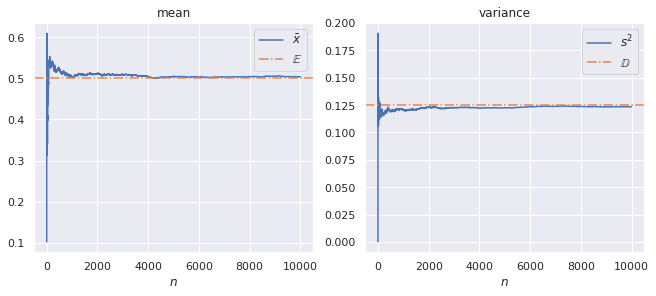
\includegraphics[width=1.0\textwidth]{resources/task2_meanvar.png}
            \caption{}
            \label{task2_meanvar}
        \end{figure}
\section{Задание 3}

\begin{enumerate}
	\item Построить датчик экспоненциального распределения. Проверить для 
    данного распределения свойство отсутствия памяти. Пусть 
    $X_1,X_2,\dots,X_n$~--- независимые экспоненциально распределенные с.в. с 
    параметрами $\lambda_1, \lambda_2, \dots, \lambda_n$ соответственно. Найти 
    распределение случайной величины $Y = \min(X_1, X_2, \dots, X_n)$.
	\item На основе датчика экспоненциального распределения построить датчик 
    пуассоновского распределения.
	\item Построить датчик пуассоновского распределения как предел биномиального
     распределения. С помощью критерия хи-квадрат Пирсона убедиться, что получен
     датчик распределения Пуассона.
	\item Построить датчик стандартного нормального распределения методом 
    моделирования случайных величин парами с переходом в полярные координаты. 
    Проверить при помощи $t$-критерия Стьюдента равенство математических 
    ожиданий, а при помощи критерия Фишера равенство дисперсий.  
\end{enumerate}

\subsection{Экспоненциальное распределение} \label{exp_section}
    Случайная величина $\epsilon$ имеет экспоненциальное распределение с 
    параметром $\lambda$, если ее функция распределения имеет вид
    \begin{equation}
        F(x) = \left\{  \begin{aligned}
            1 - e^{-\lambda x},&\quad x \ge 0,\\
            0,&\quad x < 0.
                        \end{aligned}\right.
    \end{equation}
    Мы будем моделировать $\epsilon \sim \mathrm{Exp}(\lambda)$ с помощью 
    метода обратной функции
    \footnote{см. \cite{NMS} гл. 4 \S 1 ``Метод обратной функции''.},
    согласно которому 
    \[\epsilon \sim -\frac{1}{\lambda} \ln\eta,\]
    где $\eta \sim \mathrm{Uni}\inter{0}{1}$.
    Результат моделирования см. рис. \ref{task3_exp}
    \newpage
    Экспоненциальное распределение обладает свойством отсутствия памяти 
    (рис. \ref{task3_memoexp}), т.е. аналогично \S\,\ref{par12}:
    \[\bigl. \epsilon_m \sim \epsilon ,\quad \forall{m} \in \mathbb{N} \cup \{0\},\]
    где $\epsilon_m := (\gamma \bigr|_{\Omega_m} - m),\: 
    \Omega_m = \epsilon^{-1}(\epsilon \geqslant m) \in \mathcal{A}.$ 
    \bigskip

    \begin{figure}[tbp]
        \centering
        \begin{subfigure}[b]{0.4\textwidth}
            \centering
            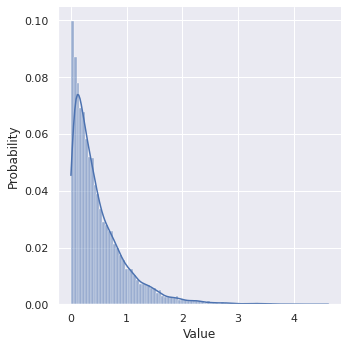
\includegraphics[width=\textwidth]{resources/task3_exp.png}
            \caption{Э.ф.п. экспоненциального распределения}
            \label{task3_exp}
        \end{subfigure}
        \hfill
        \begin{subfigure}[b]{0.5\textwidth}
            \centering
            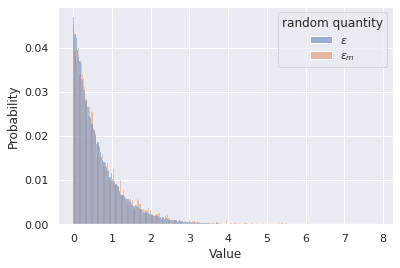
\includegraphics[width=\textwidth]{resources/task3_memoexp.png}
            \caption{Отсутствие памяти ($m = 2$)}
            \label{task3_memoexp}
        \end{subfigure}
        \caption{}
    \end{figure}

    Распределение сл.в. $Y = \min(X_1,X_2,\ldots X_n)$ имеет функцию 
    распределения 
    \begin{multline*}
        F(y) = \Prb{Y < y} = 1 - \Prb{Y \ge 1} = 
        1 - \Prb{\min(X_1,X_2,\ldots X_n) \ge 1} = \\
        1 - \Prb{X_1 \ge y, \ldots, X_n \ge y} = 
        \text{\{в силу независимости сл.в. $X_i$\} } = 
        1 - \prod_{i=1}^{n} \Prb{X_i \ge y} = \\
        1 - \prod_{i=1}^{n} (1 - F_{Exp(\lambda_i)}) = 
        1 - \prod_{i=1}^{n} (1 - (1 - e^{-\lambda_i y})) =
        1 - \prod_{i=1}^{n} e^{-\lambda_i y} = 
        1 - e^{-(\sum_{i=1}^{n} \lambda_i) y}.
    \end{multline*}
    Таким образом
    \[Y \sim \mathrm{Exp}(\sum_{i=1}^{n} \lambda_i)\]
    Cравните результаты, посчитанные для обоих представлений $Y$ 
    на рис. \ref{task3_minexp}.

    \begin{figure}[tbp]
        \centering
        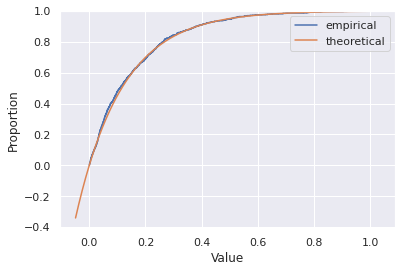
\includegraphics[width=0.7\textwidth]{resources/task3_minexp.png}
        \caption{Э.ф.р. $\mathrm{Exp}(\lambda)$}
        \label{task3_minexp}
    \end{figure}

\subsection{Датчик пуассоновского распределения 1}
    Случайная величина $\pi$ имеет распределение Пуассона с параметром 
    $\lambda > 0$, если $\Prb{\pi = k} = \dfrac{\lambda^k}{k!} e^{-\lambda}$.
    Для $\pi \sim \mathrm{Pois}(\lambda)$ верно следующее представление
    \footnote{см. \cite{NMS} гл. 5 \S 1 ``Моделирование дискретных величин''.}
    \[\pi = \max_{\mathbb{N}\cup\{0\}}(n \mid S_n = \sum_{i=1}^{n} \epsilon_i \le 1),\]
    где $\epsilon_1,\epsilon_2,\ldots$~--- экспоненциальные с параметром $\lambda$ 
    н.о.р.с.в. 

    Результат моделировния см. рис. \ref{task3_pois1}

\subsection{Датчик пуассоновского распределения 2}
    Известно, что распределение $\mathrm{Pois}(\lambda)$ получается из 
    биномиального $\mathrm{Bin}(n,p)$ предельным переходом при $n\rightarrow 
    \infty$, $p \rightarrow 0$, $np \rightarrow \lambda$. Результат моделирования 
    распределения пуассона на основе этого приниципа предоставлен на рис. \ref{task3_pois2}.

    \begin{figure}[tbp]
        \centering
        \begin{subfigure}[b]{0.48\textwidth}
            \centering
            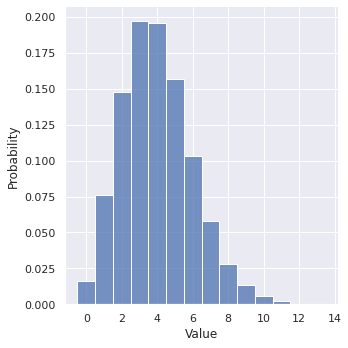
\includegraphics[width=\textwidth]{resources/task3_pois1.png}
            \caption{}
            \label{task3_pois1}
        \end{subfigure}
        \hfill
        \begin{subfigure}[b]{0.48\textwidth}
            \centering
            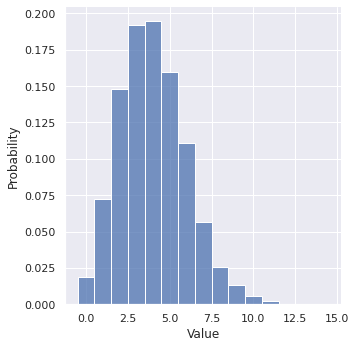
\includegraphics[width=\textwidth]{resources/task3_pois2.png}
            \caption{}
            \label{task3_pois2}
        \end{subfigure}
        \caption{Гистограммы датчиков распределения Пуассона}
    \end{figure}

    Проверим корректность нашего датчика при помощи критерия хи-квадрат Пирсона.

    Пусть $X_1,\ldots X_n$~--- выборка. Разобьем множество значений $\xi_1$ на 
    $N$ промежутков (возможно, бесконечных) $\Delta_j = (a_j, b_j], 
    j = 1,\ldots N.$ Положим $p_j = \Prb{X_1 \in \Delta_j}$, а случайные 
    величины $\nu_j$~--- равными количеству элементов выборки в $\Delta_j$.
    
    \newpage
    Так, статистикой критерия Пирсона служит величина 
    \begin{equation}
        X_n^2 = \sum\limits_{j=1}^N \dfrac{(\nu_j - n p_j)^2}{p_j},
    \end{equation}
    предел которой, при $n\rightarrow \infty$ имеет распределение $\chi_{N-1}^2$.

    Поскольку распределение Пуассона дискретно, промежутки $\Delta_j$ зададим 
    как $\Delta_j = \{j-1\}, j = 1,\ldots, N-1;\quad 
    \Delta_N = \{j\in \mathbb{N}: j > N-1\}$. $N$ положим равным приблизительно 
    $\log_2 n$. Теперь вычислим соответствующие частоты, вероятности и 
    статистику. По результатам вычислений гипотеза о корректности принимается с 
    уровнем значимости 5\%.

\subsection{Датчик стандартного нормального распределения 1} \label{3.4}
    Нормальное распределение~--- абсолютно непрерывное распределение с 
    плотностью $p(x) = \frac{1}{\sigma \sqrt{2\pi}} 
    e^{-\frac{1}{2}(\frac{x-\mu}{\sigma})^2}$, где параметры $\mu, \sigma$~--- 
    математическое ожидание и среднеквадратическое отклонение соответственно.

    С помощью нелинейного преобразования пары н.о.р.с.в. $\eta_1, \eta_2 \sim 
    \mathrm{U}\segm{0}{1}$ можно получить две н.о.р.с.в. $X,Y \sim \mathcal{N}(0,1)$:
    \begin{gather*}
        X = -\sqrt{-2\ln\eta_1}\cos(2\pi\eta_2),\\  
        Y = -\sqrt{-2\ln\eta_1}\sin(2\pi\eta_2). 
    \end{gather*}
    Результат cмоделированной таким способом стандартной нормальной случайной 
    величины см. \ref{task3_norm}.

    \begin{figure}[tbp]
        \centering
        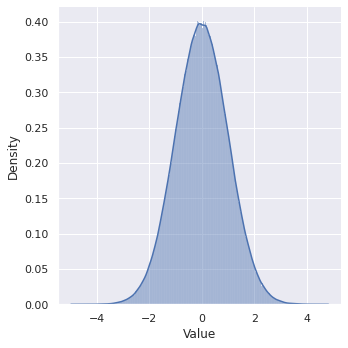
\includegraphics[width=0.5\textwidth]{resources/task3_norm.png}
        \caption{Э.ф.п. нормального распредления}
        \label{task3_norm}
    \end{figure}


    Для проверки однородности двух независимых нормальных выборок (в нашем 
    случае это $X$ и $Y$) используют критерии Фишера и Стьюдента. Оба критерия 
    имеют двустороннюю критическую области, т.о. при заданном уровне значимости 
    $\alpha$ нулевая гипотеза принимается в случае если статистика приняла 
    значение между $(\alpha/2)$ и $(1-\alpha/2)$ квантилями соответствующего 
    распределения.

    Критерий Фишера служит для проверки гипотезы о соответствии дисперсий 
    двух распределений. Его статистика имеет вид
    \begin{equation}\label{Fischer}
        \dfrac{S_1^2}{S_2^2} = \dfrac{\frac{1}{n-1}\sum_{i=1}^n (X_i-\overline X)^2}
        {\frac{1}{m-1}\sum_{j=1}^m (Y_j-\overline Y)^2},
    \end{equation}
    и распределена по закону $F_{n-1,m-1}$, т.е так же как и случайная величина 
    $\zeta~=~(\frac{1}{n-1}\xi)/(\frac{1}{m-1}\eta)$, где $\xi \sim \chi_{n-1}^2,
    \eta \sim \chi_{m-1}^2$, $\xi$ и $\eta$ независимы.
    
    В результате вычисления статистики \eqref{Fischer} гипотеза о соответствии 
    дисперсий принимается с уровнем значимости $\alpha = 5\%$.

    Критерий Стьюдента позволяет проверить гипотезу о соответствии математических
    ожиданий. Статистика в данном случае имеет вид
    \begin{equation}
        \frac{\sqrt{\frac{nm}{n+m}}(\overline X - \overline Y) (n+m-2)} 
        {[(n-1)S_1^2 + (m-1)S_2^2]} \sim t_{n+m-2},
    \end{equation}
    где $t_{n+m-2}$~--- распределение Стьюдента с $(n+m-2)$ степенями свободы.

    Значение статистики Стьюдента позволяет нам принять гипотезу о равенстве 
    мат. ожиданий с уровнем значимости $\alpha = 5\%$, что, в совокупности с уже
    установленным равенством дисперсий дает нам сделать вывод об 
    однородности нормальных выборок $X$ и $Y$ с тем же уровнем значимости.


\section{Задание 4}

\begin{enumerate}
    \item Построить датчик распределения Коши. 
    \item На основе датчика распределения Коши с помощью метода фон Неймана построить датчик стандартного нормального распределения. При помощи функции normal probabitity plot убедиться в корректности построенного датчика и обосновать наблюдаемую линейную зависимость.
    \item Сравнить скорость моделирования стандартного нормального распределения в заданях 3 и 4.
\end{enumerate}

\subsection{Датчик распределения Коши}
    Распределение Коши~--- асбсолютно непрерывное распределение с функцией 
    распределения $F(x) = \frac{1}{2} + 
    \frac{1}{\pi}\arctg(\frac{x-x_0}{\gamma})$.

    Как и в пункте \ref{exp_section} воспользуемся методом 
    обратной функции:
    \begin{equation*}
        \xi \sim F^{-1}(\eta),
    \end{equation*}
    где $\eta \sim \mathrm{U}(0,1)$, 
    $F^{-1}(y)~=~x_0+\gamma\tg[\pi(x-\frac{1}{2})]$.

    Пример результата работы полученного датчика представлен на рис. 
    \ref{cauchy}.

    \begin{figure}[tbp]
        \centering
        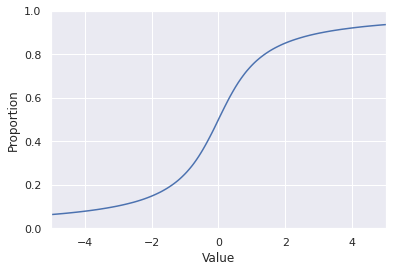
\includegraphics[width=0.5\textwidth]{resources/task4_cauchy.png}
        \caption{Э.ф.р. датчика Коши}
        \label{cauchy}
    \end{figure}

\subsection{Датчик стандартного нормального распределения 2} \label{4.2}
    Будем генерировать стандартную нормальную случайную величину методом 
    Фон-Неймана используя стандартное распределение Коши 
    ($\eta \sim \mathrm{Cauchy}(0,1)$) и распределение Бернулли.

    Требуемая выборка $\{X_i\}_{i=1}^n$ получается следующим образом. Для очередного $i$
    генерируется некоторое значение $x$ из закона $\eta \sim \mathrm{Cauchy}(0,1)$
    до тех пор, пока результат проведенного затем испытания Бернулли $\nu(x)$ с 
    вероятностью успеха $\frac{\sqrt{e}}{2} e^{-\frac{x^2}{2}} (x^2+1)$ не 
    будет положительным. Тогда значение элемента выборки $X_i$ принимается 
    равным $x$.

    Формула вероятности успеха в испытании Бернулли возникает как отношение
    "вероятностей попадания в точку $x$"$~$моделируемого распределения 
    (нормального) и распределения с помощью которого моделируют 
    (в нашем случае Коши), т.е. отношение плотностей 
    упомянутых распределений $\dfrac{p_1(x)}{p_2(x)}$. Здесь 
    $p_1(x) = \frac{1}{\sqrt{2\pi}}e^{-\frac{x^2}{2}}$, 
    $p_2(x) = \frac{1}{\pi}\frac{1}{x^2 + 1}$. Для ускорения работы 
    моделирующего алгоритма это отношение стараются приблизить к едиинце. 
    В данном случае это достигается домножением на коэффицинт $\dfrac{1}{k}$, 
    где $k = \sqrt{\dfrac{2\pi}{e}}$. В итоге получаем $p = 
    \dfrac{p_1(x)}{k p_2(x)} = \frac{\sqrt{e}}{2} e^{-\frac{x^2}{2}} (x^2+1)$.

    Для проверки корректности построенного датчика воспользуеся функцией 
    \texttt{scipy.stats.probplot}, которая строит теоретическую 
    (для стандартного нормального распределения) и эмпирическую 
    (для проверяемого распределения) функцию квантилей распределения. Поскольку 
    нормальное распредление для разных параметров линейно выражается через 
    стандратное, неудивительно что для разных $\mu$ и $\sigma$ график будет 
    меняться линейно. График для датчика стандартного нормального распределения 
    см. рис. \ref{normplot}.

    \begin{figure}[tbp]
        \centering
        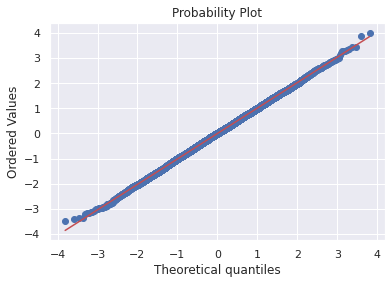
\includegraphics[width=0.5\textwidth]{resources/task4_normplot.png}
        \caption{}
        \label{normplot}
    \end{figure}

\subsection{Сравнение реализаций датчика стандартного нормального распределения}
    По результам 1000 запусков функций генерации выборки размера 1000 среднее
    время работы составляет
    \begin{itemize}
        \item $555\mu s \pm 28.6 \mu s$ для датчика из \ref{4.2}
        \item $83.6\mu s \pm 5.61 \mu s$ для датчика из \ref{3.4}
    \end{itemize}
\section{Задание 5}

\begin{enumerate}
	\item Пусть $X_i \sim \mathcal{N}(\mu, \sigma^2)$. Убедиться эмпирически в 
	справедливости ЗБЧ и ЦПТ, т.е. исследовать поведение суммы $S_n$ и 
	эмпирического распределения величины
	\begin{equation*}
		\frac{S_n - \mu n}{\sigma \sqrt{n}}.
	\end{equation*}
	\item Считая $\mu$ и $\sigma^2$ неизвестными, для пункта 1 построить 
	доверительные интервалы для среднего и дисперсии.
	\item Пусть $X_i \sim K(a, b)$ имеет распределение Коши со сдвигом $a$ и 
	масштабом $b$. Проверить эмпирически, как ведут себя суммы $S_n/n$. 
	Результат объяснить, а также найти закон распределения данных сумм.
\end{enumerate}

\subsection{Проверка ЗБЧ и ЦПТ}
	Действительно, для выборки $\{X_i\} \sim \mathcal{N}(\mu,\sigma^2)$ значение 
	$\dfrac{S_n}{n} = \dfrac{\sum_{i=1}^n X_i}{n}$ ведет себя в соответствии с 
	законом больших чисел (см. рис. \ref{LLN}), т.е
	\begin{equation*}
		\frac{S_n}{n} \rightarrow \mu \text{, при } n \rightarrow \infty.
	\end{equation*}

	Результаты опыта соответствуют и центральной пределной теореме, т.е
	\begin{equation*}
		\frac{S_n - \mu n}{\sigma \sqrt{n}} \xrightarrow{d} \eta \sim 
		\mathcal{N}(0,1) \text{ при } n \rightarrow \infty. 
		\text{ (см. рис. \ref{CLT})}
	\end{equation*}

	\begin{figure}[tbp]
        \centering
        \begin{subfigure}[b]{0.45\textwidth}
            \centering
            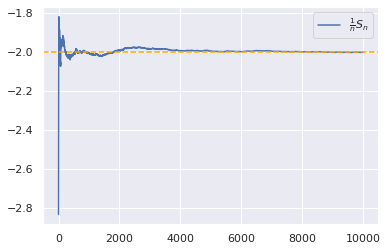
\includegraphics[width=\textwidth]{resources/task5_LLN.png}
            \caption{ЗБЧ ($\mu = -2,\:\sigma^2 = 0.5$)}
            \label{LLN}
        \end{subfigure}
        \hfill
        \begin{subfigure}[b]{0.5\textwidth}
            \centering
            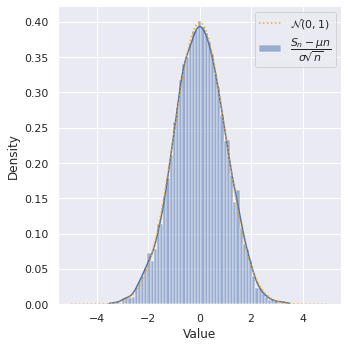
\includegraphics[width=\textwidth]{resources/task5_CLT.png}
            \caption{ЦПТ ($\mu = -2,\:\sigma^2 = 0.5$)}
            \label{CLT}
        \end{subfigure}
        \caption{}
    \end{figure}
	
\subsection{Доверительные интервалы}
	Пусть имеется выборка $X_i \sim \mathcal{N}(\mu, \sigma^2)$, где $\mu$ и 
	$\sigma^2$~--- неизвестны. Исходя из
	\begin{theorem} Для нормальной выборки $X_i \sim \mathcal{N}(\mu, \sigma^2)$
	выборочное среднее $\overline X = \frac{1}{n}\sum X_i$ и выборочная 
	дисперсия $S^2 = \frac{1}{n}\sum (X_i-\overline X)^2$ независимы, причем 
	$nS^2/\sigma^2 \sim \chi_{n-1}^2$, а $\sqrt{n-1}(\overline X - \mu)/S 
	\sim t_{n-1}$.
	\end{theorem}
	можно построить доверительные интервалы 
	\begin{itemize}
		\item для параметра сдвига $\mu$:
		\[\Prb{\overline X - \frac{y_{1-\alpha/2}S}{\sqrt{n-1}} < \mu < 
		\overline X - \frac{y_{\alpha/2}S}{\sqrt{n-1}}} = 
		\Prb{y_{\alpha/2} < \frac{\sqrt{n-1}(\overline X - \mu)}{S} < 
		y_{1-\alpha/2}} = 1-\alpha,\]
		где $y_p$~--- $p$-квантиль распределения Стьюдента $t_{n-1}$ (в силу 
		симметрия закона $y_{\alpha/2} = -y_{1-\alpha/2}$);
		\item и для параметра масштаба $\sigma$:
		\[\Prb{\frac{\sqrt{n}S}{\sqrt{z_{1-\alpha/2}}} < \sigma < 
		\frac{\sqrt{n}S}{\sqrt{z_{\alpha/2}}}} = \Prb{z_{\alpha/2} < 
		\frac{nS^2}{\sigma^2} < z_{1-\alpha/2}} = 1-\alpha,\]
		где $z_p$~--- $p$-квантиль закона $\chi_{n-1}^2$.
	\end{itemize}

	Доверительные интервалы для некотрой выборки из $\mathcal{N}(-2,0.5)$ для 
	разных $n$ приведены на рис. \ref{CI}	

	\begin{figure}[tbp]
        \centering
        \begin{subfigure}[b]{0.47\textwidth}
            \centering
            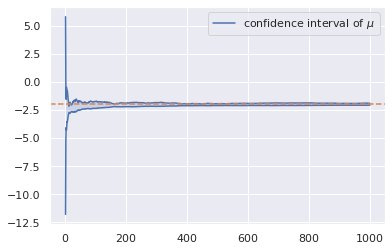
\includegraphics[width=\textwidth]{resources/task5_CI_mu.png}
            \caption{}
            \label{CI_mu}
        \end{subfigure}
        \hfill
        \begin{subfigure}[b]{0.45\textwidth}
            \centering
            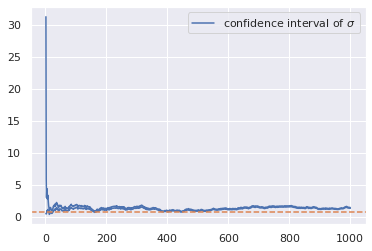
\includegraphics[width=\textwidth]{resources/task5_CI_sigma.png}
            \caption{}
            \label{CI_sigma}
        \end{subfigure}
        \caption{} \label{CI}
    \end{figure}

\subsection{Поведение сумм $S_n/n$ для распределения Коши}
	Как известно распределение Коши не имеет математического ожидания (ни 
	конечного, ни бесконечного), а потому для него не выполяется ЗБЧ, и 
	сходимость выборочного среднего $S_n/n$ не имеет места. Тем не менее 
	распределение $\mathrm{Cauchy}(a,b)$ симметрично относительно $a$ и интеграл 
	$\int\limits_{-\infty}^{\infty} x p_{c}(x)\, dx$ сходится  в смысле главного 
	значения к $a$. Этими наблюденями объясняется полученное на опыте поведение
	сумм $S_n/n$: их значение в основном держится около некоторой средней 
	величины определяемой значением $a$ (сходимость $v.p.$) и "периодическими" 
	сильными выборосами (расходимость в целом) от $a$ ее отклонившими. График 
	сумм $S_n/n$ для некоторой выборки $X_i$ представлен на 
	рис. \ref{cauchy_sums}.

	\begin{figure}[tbp]
        \centering
        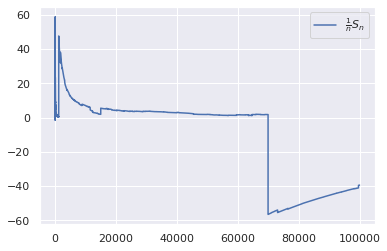
\includegraphics[width=0.5\textwidth]{resources/task5_cauchy.png}
        \caption{$a=0, b=3$}
        \label{cauchy_sums}
    \end{figure}

	Ввиду отстутствия математического ожидания не выполнена и ЦПТ, и сходимость 
	$S_n/n$ по распределению с ее помощью доказать не получится. Вместо этого 
	воспользуемся аппаратом характеристических функций. Характеристическая 
	функция распределения Коши с параметрами $a$, $b$ имеет вид
	\begin{equation*}
		\psi(t) = 
		\int\limits_{-\infty}^{\infty} \frac{e^{itx}}{\pi(b^2 + (x-a)^2)} \,dx =
		e^{ait-b|t|}.
	\end{equation*}
	Характеристическая функция суммы независимых случайных величин есть 
	произведение их характеристических функций, а потому
	\begin{equation} \label{char_fun}
		\psi_{\frac{S_n}{n}}(t) = \psi_{\sum \frac{1}{n} X_i} (t) = 
		\prod \psi_{\frac{1}{n} X_i} (t) = \prod \psi_{X_i} (\tfrac{t}{n}) = 
		e^{n(ai\frac{t}{n}-b|\frac{t}{n}|)} = e^{ait-b|t|}.
	\end{equation}
	Поскольку хар. функция однозначно задает распределение, равенство 
	\eqref{char_fun} доказывет что величина $\frac{S_n}{n}$ (так же как и 
	${X_i}$) распределена по Коши с параметрами $a$ и $b$.
\section{Задание 6}

\begin{enumerate}
	\item Посчитать интеграл
	\begin{equation}\label{integral}
	\int\limits_{-\infty}^{\infty} \int\limits_{-\infty}^\infty \cdots \int\limits_{-\infty}^\infty \frac{e^{-\left(x_1^2 + \ldots + x_{10}^2 + \frac{1}{ 2^7\cdot x_1^2 \cdot \ldots \cdot x_{10}^2}\right)}}{x_1^2 \cdot \ldots \cdot x_{10}^2}\,dx_1 dx_2 \ldots dx_{10}
	\end{equation}
	\begin{itemize}
		\item[---] методом Монте-Карло
		\item[---] методом квадратур, сводя задачу к вычислению собственного интеграла Римана
	\end{itemize}
	\item Для каждого случая оценить точность вычислений.
\end{enumerate}

\subsection{Численное интегрирование}
	Перепишем \eqref{integral} следующим образом
	\begin{multline*}
	\idotsint_{\mathbb{R}^{10}} \frac{e^{-\left(x_1^2 + \ldots + x_{10}^2 + 
	\frac{1}{ 2^7\cdot x_1^2 \cdot \ldots \cdot x_{10}^2}\right)}}
	{x_1^2 \cdot \ldots \cdot x_{10}^2}\,dx_1 dx_2 \ldots dx_{10} = \\
	\idotsint_{\mathbb{R}^{10}} 
	\frac{\pi^5 e^{-\frac{1}{ 2^7\cdot x_1^2 \cdot \ldots \cdot x_{10}^2}}}
	{x_1^2 \cdot \ldots \cdot x_{10}^2} \cdot 
	\frac{e^{-(x_1^2 + \ldots + x_{10}^2)}}{\pi^5}\,dx_1 dx_2\ldots dx_{10} = 
	\idotsint_{\mathbb{R}^{10}} f(x) \cdot p(x)\,dx,
	\end{multline*}
	где $p(x)$~--- плотность многомерного нормального распределения 
	$\mathcal{N}(0,\frac{1}{2} E)$,\\ $E\in \mathbb{R}^{10\times10}$. Таким образом
	\begin{equation*}
		\idotsint_{\mathbb{R}^{10}} f(x) \cdot p(x)\,dx = \Exp{f(\eta)}, \quad
		\eta \sim \mathcal{N}(0,\frac{1}{2} E).
	\end{equation*}

	По усиленному закону больших чисел имеем
	\begin{equation*}
		\widehat I_n = \frac{1}{n}\sum\limits_{i=1}^{n} f(\eta_i) 
		\xrightarrow[]{\text{п.н.}} \Exp f(\eta) =
		\idotsint_{\mathbb{R}^{10}} f(x) \cdot p(x)\,dx = I,
	\end{equation*}
	что дает нам основания использовать метод Монте-Карло для вычисления 
	интеграла \eqref{integral}.

	Другим способом вычисления может служить метод квадратур, для реализации 
	которого проведем замену
	\begin{equation*}
		x_i = \tg (\tfrac{\pi}{2}t_i),\: t_i \in [0,1],\quad i = \overline{1,10}.
	\end{equation*}
	Тогда \eqref{integral} примет вид 
	\begin{equation}\label{Rint}
		I = \pi^{10} \idotsint_{[0,1]^{10}} \frac
		{e^{-\biggl(\textstyle{ \sum\limits_{i=1}^{10} \tg (\frac{\pi}{2}t_i)^2 + 
		\frac{1}{2^7 \prod_{i=1}^{10}\tg(\frac{\pi}{2}t_i)^2} }\biggr)}}
		{\prod_{i=1}^{10}\tg(\frac{\pi}{2}t_i)^2 \cdot 
		\prod_{i=1}^{10}\cos(\frac{\pi}{2}t_i)^2} \, dt.
	\end{equation}
	Интeграл \eqref{Rint} уже можно вычислить, например, стандартным методом 
	прямоугольников на равномерной сетке.

\subsection{Точность вычислений}
	В соответствии с ЦПТ и правилом трех сигм, при достаточно больших $n$ 
	погрешность метода Монте-Карло с вероятностью около $0.997$ составляет
	\begin{equation*}
		\psi_n = 3\frac{\sqrt{\Disp{f(\eta)}}} {\sqrt{n}} \ge |\hat I_n - I|.
	\end{equation*}
	Для вычисления погрешности будем приближать значение $\Disp{f(\eta)}$ 
	выборочной дисперсией 
	\begin{equation*}
		S_n^2 = \frac{1}{n} \sum_{i = 1}^n f^2(x_i) - \left( \frac{1}{n}
 \sum_{i = 1}^n f(x_i) \right)^2.
	\end{equation*}
	Результаты работы программы представлены на таблице \ref{tabMC}.
	
	\begin{table}[ht]
	\begin{tabular}{|cccc}
		Объем выборки & Результат & Величина ошибки & Время работы (сек.) \\[5pt]
		$n=10^3$      & 120.0206  & 13.7449         & 0.021               \\
		$n=10^4$      & 122.5785  & 3.3040          & 0.416                \\
		$n=10^5$      & 124.7199  & 1.0937          & 3.67                 \\
	\end{tabular}
	\caption{}
	\label{tabMC}
	\end{table}
	
	Как известно погрешность метода прямоугольников составляет 
	\begin{equation*}
		\psi_n = \frac{h^2}{24} (b-a) \sum\limits_{i,j = 1}^{10} 
		\max |f''_{x_i x_j} | = 
		\frac{1}{6n^2} \sum\limits_{i,j = 1}^{10} \max |f''_{x_i x_j} |.
	\end{equation*}
	Результаты работы программы см. на таблице \ref{tabRS}.

	\begin{table}[ht]
	\begin{tabular}{|ccc}
		Мощность сетки & Результат  & Время работы (сек.) \\[5pt]
		$n=10^3$       & 1572.5830  & 0.03                \\
		$n=10^4$       & 1247.9712  & 0.474               \\
		$n=10^5$       & 794.7241   & 5.19                \\
	\end{tabular}
	\caption{}
	\label{tabRS}
	\end{table}
\newpage
\section{Задание 7}

\begin{enumerate}
	\item Методом случайного поиска найти минимальное значение функции $f$ на 
    множестве $A = \{x_1, x_2 : x_1^2 + x_2^2 \leq 1\}$, т.е. $y = \min f(x)$, 
    где 
    \begin{equation*}
        f(x) = x_1^3\sin\left(\frac{1}{x_1}\right) + 
        10x_1 x_2^4\cos\left(\frac{1}{x_2}\right)
    \end{equation*}
    при $x_1 \neq 0$ и $x_2 \neq 0$, функция доопределяется по непрерывности 
    при $x_1 = 0$ или $x_2 = 0$.
    \item Методом имитации отжига найти минимальное значение функции Розенброка 
    $g$ в пространстве $\mathbb{R}^2$, где 
    \begin{center}
	    $g(x) = (x_1-1)^2+100(x_2-x_1^2)^2$
    \end{center}
    \item Оценить точность. Сравнить результаты со стандартными методами 
    оптимизации.
\end{enumerate}

\subsection{Случайный поиск}
    Случайный поиск релизуем следующим образом. Равномерно разбросаем на 
    единичном круге $A$ точки $(X_i,Y_i) \sim \mathrm{Uniform}(A)$, т.е.
    \begin{gather*}
        X_i = \sqrt{r} \cos(\phi),\\
        Y_i = \sqrt{r} \sin(\phi),
    \end{gather*}
    где $r \sim \mathrm{Uniform}[0,1], \phi \sim \mathrm{Uniform}[0,2\pi]$. Из 
    полученной выборки возьмем точку $(X_k,Y_k)$ доставляющюю минимум функции 
    $f$. Она и будет результатом работы алгоритма. Испытания см. таб. 
    \ref{randsearch}.

    \begin{table}[ht]
        \begin{tabular}{|cccc}
            Объем выборки & $argmin$           & $min$   \\[5pt]
            $n=10^3$      & ( 0.4135, -0.9091) & -1.2351 \\
            $n=10^4$      & (-0.3691, -0.9256) & -1.2557 \\
            $n=10^5$      & (-0.3472, -0.9372) & -1.2832 \\
            $n=10^6$      & (-0.3576, -0.9338) & -1.2883 \\
        \end{tabular}
        \caption{}
        \label{randsearch}
    \end{table}

\subsection{Отжиг}
        Алгоритм метода принимает некоторую точку $x_0$ как исходные данные. 
        Затем строится минимизирующая последовательность $\{x_i\}$. Точка $x_{i+1}$ 
        полчучается на основе текущей точки $x_i$, а именно: случайно 
        генерируется точка $x^*$, например из распределения 
        $\mathcal{N}(x_i,q_i\sigma^2 E)$, после чего точка $x^*$ с некоторой вероятностью
        становится точкой $x_{i+1}$
        \begin{equation*}
            \Prb{x^* \rightarrow x_{i+1} | x_i} = 
            \left\{\begin{aligned}
                1\quad, & F(x^*) \le F(x_i),\\
                \exp\left(-\frac{F(x^*)-F(x_i)}{q_i}\right),& F(x^*) \ge F(x_i).
            \end{aligned}\right.
        \end{equation*}
        В качестве $\{q_i\}$ берется обычно некоторая убывающая 
        последовательность, например геометрическая прогрессия со знаменателем 
        меньшим едиинцы.

        За $100$ шагов алгоритм с параметрами: $x_0 = (0,0), \sigma = 2, 
        q_0 = 1000, k = 0.93$ нашел $min = 0.0031$ в точке $x_{100} = 
        (1.0382, 1.0820)$.

\subsection{Оценка точности}
    Оценим точность случайного поиска. Пусть $x = (x_1, x_2)$~--- точка 
    минимума, $\hat{x} = (\hat{x}_1, \hat{x}_2)$ --- результат работы алгоритма.

    Вероятность того что хотя бы одна точка попадет в $\epsilon$-окрестность $x$ 
    составляет $1 - (1-2\epsilon^2)^n$. Таким образом
    \begin{equation*}
        \Prb{|x - \hat x| < \epsilon} = 1 - (1-2\epsilon^2)^n.
    \end{equation*}
    Ясно, что $|f(x) - f(\hat x)| < \|f'\||x - \hat{x}| < 
    \max_A \|f'\| |x - \hat{x}|$.
    Можно оценить $\max_A \|f'\|$ как
    \begin{equation*}
        \|f'\| = \sqrt{\left(\frac{\partial f}{\partial x_1}\right)^2 
        + \left(\frac{\partial f}{\partial x_2}\right)^2} \le  34.26.
    \end{equation*}

    Итого мы можем оценить ошибку $\psi_n = |f(x) - f(\hat x)|$ сверху величиной 
    $\epsilon$, с вероятностью $1 - (1-2(\frac{\epsilon}{34.26})^2)^n$.
\section{Задание 8}

Применить метод Монте-Карло к решению первой краевой задачи для двумерного 
уравнения Лапласа в единичном круге:
\begin{equation} \label{Dirichlet}
    \left\{
    \begin{array}{lcr}
        \Delta u = 0,(x,y) \in D,        \\
        u |_{\delta D }= f(x,y),         \\
        u \in C^2(D), f \in C(\delta D), \\
        D= \{ x,y: x^2 + y^2 \le 1 \}
    \end{array}
    \right.
\end{equation}

Для функции $f(x,y) = x^2 - y^2$ найти аналитическое решение и сравнить с 
полученным по методу Монте-Карло.

\bigskip

Численное решение уравнения Дирихле \eqref{Dirichlet} в круге $D$ можно 
получить таким способом. Для каждой точки $M$ из заданной заранее сетки $N$ 
раз проводится следующая процедура. Сначала строится окружность с центром в 
точке $M$ и максимальным радиусом, таким что эта окружность еще принадлежит 
замыканию $D$. На окружности разыгрывется случайная равномерно распределенная 
точка $M_1$. Если $\rho(M_1, \partial D) < \epsilon$, то процесс 
обрывается и выбирается граничное значение $f(Q^1)$, где $Q^1$~--- ближайшая 
граничная точка, инчаче $M_1$ принимается за следующую точку и процедура 
продолжается. 

После того как такой процесс блуждания производится $N$ раз считается среднее 
арифметическое 
\begin{equation*}
    \frac{f(Q^1) + f(Q^2) + \ldots + f(Q^N)}{N},
\end{equation*}
являющееся приближенным значением искомого решения $u(M)$.

Аналитическим решением \eqref{Dirichlet} для $f(x,y) = x^2 - y^2$ является, 
очевидно, $u~=~x^2~-~y^2$. Сравните аналитическое решение с результатом работы 
описанного выше алгоритма на рис. \ref{dirMC}

\begin{figure}[tbp]
    \centering
    \begin{subfigure}[b]{0.48\textwidth}
        \centering
        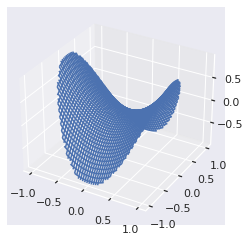
\includegraphics[width=\textwidth]{resources/task8_analytical.png}
        \caption{Аналитическое решение}
    \end{subfigure}
    \hfill
    \begin{subfigure}[b]{0.48\textwidth}
        \centering
        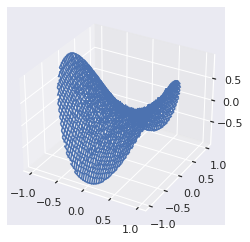
\includegraphics[width=\textwidth]{resources/task8_numerical.png}
        \caption{Численное решение ($N=1000$)}
    \end{subfigure}
    \caption{}
    \label{dirMC}
\end{figure}

\section{Задание 9}

Рассмотреть два вида процессов:
\begin{itemize}
	\item Винеровский процесс $W(t), t \in [0,1], W(0) = 0$.
	\item Процесс Орнштейна--Уленбека $X(t), t \in [0,1], X(0) = X_0$, то есть 
    стационарный марковский гауссовский процесс. Начальные значения $X_0$ 
    генерируются случайным образом так, чтобы полученный процесс был 
    стационарным.
\end{itemize}

Для данных гауссовских процессов
\begin{enumerate}
	\item Найти ковариационную функцию и переходные вероятности.
	\item Моделировать независимые траектории процесса с данными переходными 
    вероятностями методом добавления разбиения отрезка.
	\item Построить график траектории, не соединяя точки ломаной, с целью 
    получения визуально непрерывной линии.
\end{enumerate}

\subsection{Винеровский процесс}

    По определннию (\cite{SAIM}) ковариационная функция Винеровского процесса 
    $W_t$ имеет вид $\cov(t,s) = \min (t,s)$. Плотность многомерного 
    нормального распределения $\mathcal{N}(m,R)$
    \begin{equation*}
        p(x) = \frac{1}{(2\pi)^
        {\frac{n}{2}}\sqrt{|R|}}e^ {-\frac{1}{2}(x-m)^T R^{-1}(x-m)},
    \end{equation*}
    где $R$ --- ковариационная матрица. Для моделирования Винеровского процесса 
    достаточно знать, что $W_0 = 0, W_1 \sim \mathcal{N}(0,1)$ и для $t_0, t_1, 
    \alpha \in (0,1)$ условное распределение в момент $t = (1-\alpha)t_0 + 
    \alpha t_1$ имеет плотность
    \begin{equation*}
        p_{W_t \mid W_{t_0},W_{t_1}} (x \mid x_0,x_1) = 
        \frac{p_{W_{t_0},W_t,W_{t_1}}(x_0,x,x_1)} {p_{W_{t_0},W_{t_1}}(x_0,x_1)},
	\end{equation*}
    где
    \begin{gather*}
        p_{W_{t_0},W_t,W_{t_1}} = \frac{1}{(2\pi)^{\frac{3}{2}}\sqrt{|R_3|}} 
        e^{-\frac{1}{2}x^T R_3^{-1} x},\\
        p_{W_{t_0},W_{t_1}} = 
        \frac{1}{(2\pi)\sqrt{|R_2|}} e^{-\frac{1}{2}x^T R_2^{-1} x},\\
        R_3 = \begin{pmatrix}
                t_0 & t_0 & t_0 \\
                t_0 & t & t \\
                t_0 & t & t_1
                \end{pmatrix} ,
        R_2 = \begin{pmatrix}
            t_0 & t_0 \\
            t_0 & t_1
            \end{pmatrix}.        
    \end{gather*}

    Отсюда
    \begin{equation*}
        p_{W_t \mid W_{t_0},W_{t_1}} (x \mid x_0,x_1) = 
        \frac{1}{\sqrt{2\pi\alpha(1-\alpha)(t_1-t_0)}} 
        e^{\displaystyle{-}
        \dfrac{(x-((1-\alpha)x_0+\alpha x_1))^2}{2\alpha(1-\alpha)(t_1-t_0)}},
    \end{equation*}
    т.е. $W_t \sim \mathcal{N}(x,\alpha(1-\alpha)(t_1 - t_0))$. В случае 
    $\alpha = \frac{1}{2}$ $W_t \sim \mathcal{N}(x,\frac{t_1-t_0}{4})$

    Таким образом, для моделирования Винеровского процесса достаточно получить 
    некоторые значения $W_0 = 0$, $W_1 \sim \mathcal{N}(0,1)$, и затем 
    последовательно методом бисекции разыгрывать величины $W_t \sim 
    \mathcal{N}(x,\frac{t_1-t_0}{4})$.

\subsection{Процесс Орнштейна-Уленбека}

    Из стационарности процесса Орнштейна-Уленбека $X_t$ следует, что 
    $\Exp X_t = a$, $\Disp X_t = \sigma^2$ и
    \begin{equation*}
        \cov (X_t,X_s) = \sigma^2 \rho(x,y) = \sigma^2 \rho(x) \rho(y) = 
        \sigma^2 e^{-\theta(x+y)}
    \end{equation*}

    Условное распределение имеет вид $(X_t \mid X_s = x) \sim 
    \mathcal{N}(x e^{\theta |t-s|},\:\sigma^2(1-e^{-2\theta |t-s|}))$.

    Процесс Орнштейна-Уленбека моделируется так же как и Винеровский, лишь с 
    учетом того, что $X_0 \sim \mathcal{N}(a,\sigma^2)$, 
    $X_1 \sim \mathcal{N}(x_0 e^{-\theta T}, \sigma^2 (1-e^{-2\theta T}))$, и
    \begin{equation*}
        X_{\frac{t_0 + t_1}{2}} \sim \mathcal{N}\left( 
            (x_0+x_1)\frac{e^\frac{-\theta(t_1-t_0)}{2}}{1 + e^{-\theta(t_1-t_0)}},\:
            \sigma^2 \frac{1 - e^{-\theta(t_1-t_0)}}{1 + e^{-\theta(t_1-t_0)}} 
            \right)
    \end{equation*}

    Результат моделирования процессов см. рис. \ref{processes}

    \begin{figure}[tbp]
        \centering
        \begin{subfigure}[b]{0.48\textwidth}
            \centering
            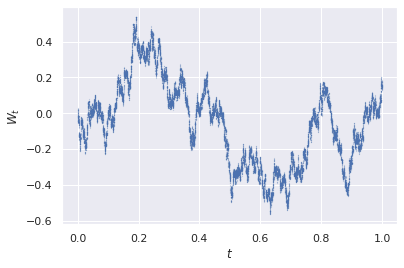
\includegraphics[width=\textwidth]{resources/task9_Wiener.png}
            \caption{Винеровский процесс}
        \end{subfigure}
        \hfill
        \begin{subfigure}[b]{0.48\textwidth}
            \centering
            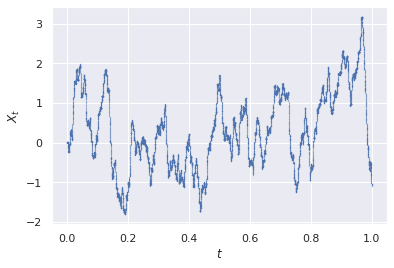
\includegraphics[width=\textwidth]{resources/task9_OrnUhl.png}
            \caption{Процесс Орнштейна-Уленбека}
        \end{subfigure}
        \caption{}
        \label{processes}
    \end{figure}
\section{Задание 10}

Произвести фильтрацию одномерного процесса Орнштейна-Уленбека:
\begin{enumerate}
    \item Используя генератор белого шума, добавить случайную ошибку с 
    известной дисперсией к реализации процесса Орнштейна-Уленбека.
	\item При помощи одномерного фильтра Калмана оценить траекторию процесса по 
    зашумленному сигналу. Параметры процесса и белого шума считать известными.
	\item Рассмотреть случай, когда шум
	\begin{itemize}
		\item Является гауссовским.
		\item Имеет распределение Коши.
	\end{itemize}
\end{enumerate}
\bigskip

Белый шум для случайного процесса $x_{k+1} = A_k x_k$ будем моделировать 
линейным стохастическим уравнением 
\begin{equation} \label{white_noise}
	 x_{k+1} = A_k x_k + \omega_k,
\end{equation}
где $\omega_k$~--- случайная помеха, распределенная нормально или по Коши.

Фильтр Калмана для задачи \eqref{white_noise} имеет вид
\begin{equation} \label{kalman_filter}
    \left\{
    \begin{array}{lcr}
        \hat x_{k\mid k} = \hat x_{k\mid k-1} + R_{k \mid k-1} 
			C_k^T (C_k R_{k\mid k-1} C_k^T + N_k)^{-1} 
			(y_k - C_k \hat x_{k\mid k-1} - \Exp v_k),        	 			\\
		\hat x_{k+1\mid k} = A_k \hat x_{k\mid k} + \Exp \omega_k, 			\\
		R_{k\mid k} = R_{k\mid k-1} - R_{k\mid k-1} 
			C_k^T (C_k R_{k\mid k-1} C_k^T + N_k)^{-1} C_k R_{k\mid k-1},	\\
		R_{k+1 \mid k} = A_k R_{k\mid k} A_k^T + M_k,						\\
		\hat x_{0\mid -1} = \overline{x_0}, R_{0\mid -1} = s,				\\
    \end{array}
    \right.
\end{equation}
где  $y_k = C_k x_k + v_k$~--- измерения, 
$x_{k+1} = A_k x_k + \omega_k$~--- шаги. В случае процесса Орнштейна-Уленбека с 
параметрами $\lambda$, $\sigma$ система \eqref{kalman_filter} принимает вид
\begin{equation}
    \left\{
    \begin{array}{lcr}
        \hat x_{k\mid k} = \hat x_{k\mid k-1} + R_{k \mid k-1} 
			(R_{k\mid k-1} \sigma_v^2)^{-1} 
			(y_k - \hat x_{k\mid k-1}),										\\
		\hat x_{k+1\mid k} = e^{-\lambda\Delta t} \hat x_{k\mid k}, 		\\
		R_{k\mid k} = R_{k\mid k-1} - R_{k\mid k-1} 
			(R_{k\mid k-1} + \sigma_v^2)^{-1} R_{k\mid k-1},				\\
		R_{k+1 \mid k} = e^{-\lambda \Delta t} R_{k\mid k} A_k^T + 
		\sigma^2 (1-e^{-2\lambda \Delta t}),								\\
		\hat x_{0\mid -1} = 0, R_{0\mid -1} = \sigma^2,						\\
    \end{array}
    \right.
\end{equation}
Доверительный интервал фильтрации состовляет
\begin{equation}
	- k_{1-\frac{\alpha}{2}}\sqrt{R_{k\mid k}} < \hat x_{k\mid k} < 
	k_{1-\frac{\alpha}{2}}\sqrt{R_{k\mid k}},
\end{equation}
где $k_{1-\frac{\alpha}{2}}$~--- $(1-\frac{\alpha}{2})$-квантиль нормального 
распределения.

Пример работы программы см рис. \ref{filter}.

\begin{figure}[tbp]
	\centering
	\begin{subfigure}[b]{0.48\textwidth}
		\centering
		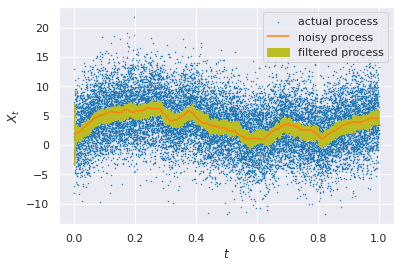
\includegraphics[width=\textwidth]{resources/task10_kalman_normal.png}
		\caption{Гауссовский шум}
	\end{subfigure}
	\hfill
	\begin{subfigure}[b]{0.48\textwidth}
		\centering
		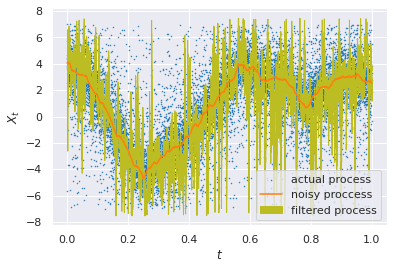
\includegraphics[width=\textwidth]{resources/task10_kalman_cauchy.png}
		\caption{Шум распределенный по Коши}
	\end{subfigure}
	\caption{Фильтрация Калмана}
	\label{filter}
\end{figure}

\newpage
\section{Задание 11}

Построить двумерное пуассоновское поле, отвечающее сложному пуассоновскому 
процессу:
\begin{enumerate}
	\item Первая интерпретация: система массового обслуживания. При этом первая 
    координата поля~---~время поступления заявки в СМО (равномерное 
    распределение), вторая~---~время её обслуживания (распределение $\chi^2$ с 
    $10$-ю степенями свободы).

	\item Вторая интерпретация: система массового обслуживания с циклической 
    интенсивностью $\lambda(t) = \lambda_0(1+\cos(t))$ и единичными скачками. 
    Свести данную задачу моделирования неоднородного пуассоновского процесса 
    при помощи метода Льюиса и Шедлера к моделированию двумерного 
    пуассоновского поля, где первая координата имеет равномерное распределение, 
    а вторая~---~распределение Бернулли.
	
	\item Третья интерпретация: работа страховой компании. Первая 
    координата~---~момент наступления страхового случая (равномерное 
    распределение), вторая координата~---~величина ущерба (распределение 
    Парето). Поступление капитала по времени линейно со скоростью $c > 0$, 
    начальный капитал $W > 0$.
	
	\item Для каждой системы рассмотреть всевозможные случаи поведения системы 
    в зависимости от значения параметров.
\end{enumerate}

\subsection{СМО}
    Систему массового обслуживания будем моделировать временами поступления 
    заявок $t_i$: $t_i - t_{i-1} \sim \mathrm{Exp}(\lambda)$, где $\lambda$~--- 
    интенсивность потока заявок, и временами обработки завявок $s_i$ 
    распределенных по закону $\chi^2$ с $10$ степенями свободы. Для каждой 
    заявки будет считаться время ее исполнения, т.е. если следуюзщая заявка 
    пришла раньше чем прошло время обработки заявки то будет накапливаться 
    очередь. Поскольку $\Exp s_i = 10$, в зависимости того, больше $\lambda$ чем
    $\frac{1}{10}$ или меньше, очередь будет в среднем накапливаться или 
    сокращаться соответственно.

\subsection{СМО с циклической интенсивностью}
    Имеющийся неоднородный процесс с помощью вышеупомянутого алгоритма сводится 
    к двумерному пуассоновскому полю, а именно, генерируется стационарный 
    пуассоновский процесс $X_t$, из множества точек роста которого случайно 
    (с бернуллиевским распределением) выбирается подмножество $T$. Совокупность 
    полученных величин образует искомое пуассоновское поле.

    Иллюстрации работы моделей СМО представлены на рис. \ref{smo} 

    \begin{figure}[tbp]
        \centering
        \begin{subfigure}[b]{0.48\textwidth}
            \centering
            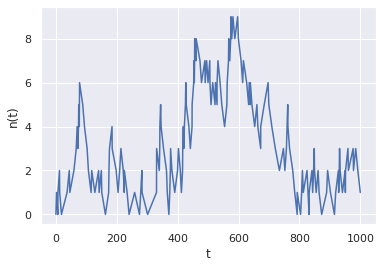
\includegraphics[width=\textwidth]{resources/task11_smo_const.png}
            \caption{с постоянной интенсивностью}
        \end{subfigure}
        \hfill
        \begin{subfigure}[b]{0.48\textwidth}
            \centering
            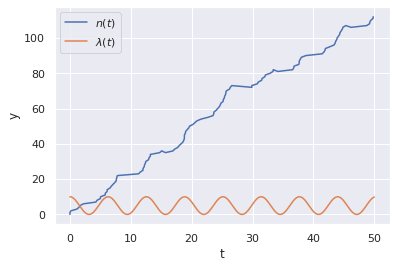
\includegraphics[width=\textwidth]{resources/task11_smo_cyclic.png}
            \caption{с циклической интенсивностью}
        \end{subfigure}
        \caption{СМО}
        \label{smo}
    \end{figure}

\subsection{Работа страховой компании}
    Для построения модели работы страховой компании генерируются времена 
    поступления страховых случаев $t_i$: $t_i - t_{i-1} \sim 
    \mathrm{Exp}(\lambda)$ и ущерб страхового случая $s_i$ распределенный по 
    Парето с параметрами $x_m$ и $k$. По ним можно вычислить величину капитала 
    компании в момент $t$: $W(t) = W_0 + cy - \sum_{i:t_i<t} s_i$ и среднюю 
    скорость прироста капитала $(\Exp W(t))' = c - \dfrac{\lambda k x_m}{k-1}$.
    Из чего можно заключить, что страховая компания будет расти при 
    $c(k-1)-\lambda k x_m > 0$, и обанкротится при $c(k-1)-\lambda k x_m < 0$.

    \begin{figure}[tbp]
        \centering
        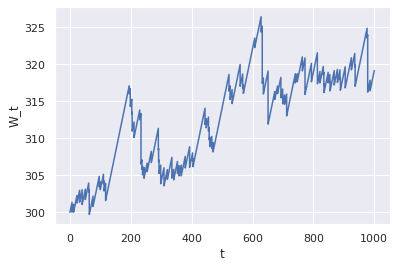
\includegraphics[width=0.5\textwidth]{resources/task11_insur_comp.png}
        \caption{работа страховой компании}
        \label{ins_comp}
    \end{figure}

\begin{thebibliography}{0}
    \bibitem{SAIM} Смирнов~С.~Н. кафедральный курс 
        \emph{"<Стохастический анализ и моделирование">}, 2021.
    \bibitem{SHIR} Ширяев~A.~Н. 
        \emph{"<Вероятность">}. Изд-во Наука, Москва, 1979.
    \bibitem{NMS} Лагутин~М.~Б.
        \emph{"<Наглядная математическая статистика">}. Изд-во Бином, Москва, 2009.
    \bibitem{MC} Бусленко~Н.~П., Шрейдер~Ю.~А.
        \emph{"<Метод статистических испытаний">}. Изд-во физ-мат литературы, Москва, 1961.         
\end{thebibliography}

\end{document}